\begin{figure}[H]
    \centering
    \begin{subfigure}[b]{\textwidth}
        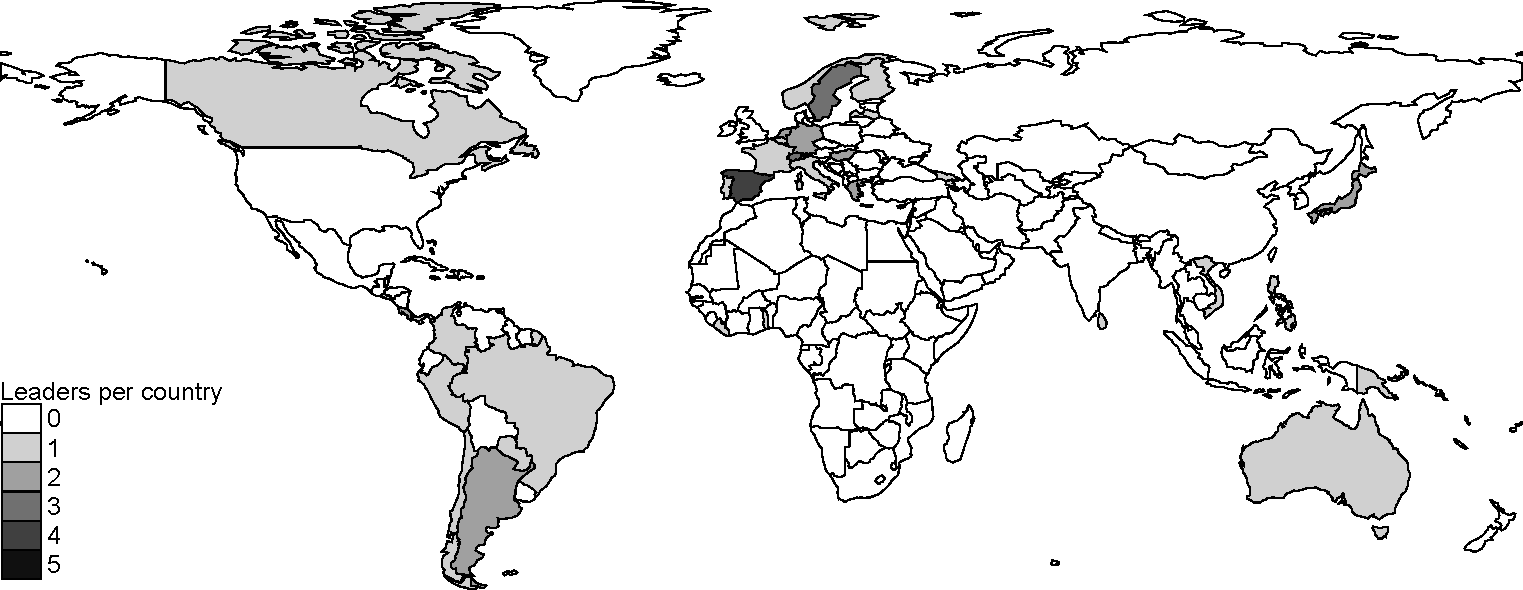
\includegraphics[width=\textwidth]{Figures/World50ex_vsimple.pdf}
        \caption{Distribution of leaders across countries}
        \label{fig:world_map_50}
    \end{subfigure}
    \\ %add desired spacing between images, e. g. ~, \quad, \qquad, \hfill etc. 
      %(or a blank line to force the subfigure onto a new line)
    \begin{subfigure}[b]{0.8\textwidth}
        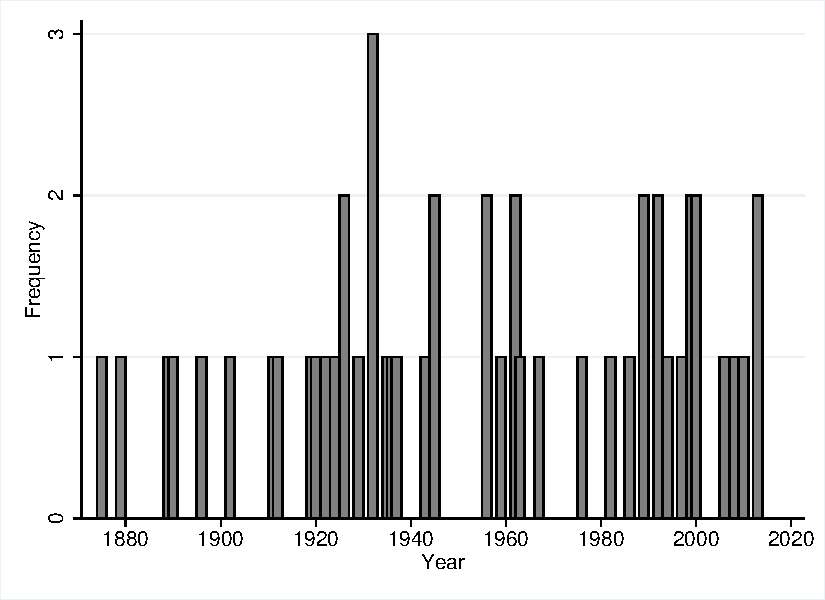
\includegraphics[width=\textwidth]{Figures/Year_50ex.pdf}
        \caption{Distribution of leaders in time}
        \label{fig:timeline_50}
    \end{subfigure}
    %~ %add desired spacing between images, e. g. ~, \quad, \qquad, \hfill etc. 
    %(or a blank line to force the subfigure onto a new line)
    \caption{Distribution of leaders with regular transitions}
    \label{fig:robust_dist}
    \medskip % induce some separation between caption and explanatory material
   % \begin{minipage}{\textwidth} % choose width suitably
    	%{\footnotesize  Notes:  The map above shows the distribution of leaders with random transitions in our sample across countries. The timeline below shows how leaders with random transitions are distributed in time. The earliest random transition is in 1875, the latest in 2012.  \par}
    %\end{minipage}
\end{figure}
